\scanpage{55}
\mspage{\handwritten{23}}
% archive sheet number: 54

$\handwritten{\rho}(e_{\unsure{o|0}})=\handwritten{\sum}a_i\handwritten{\otimes}e_i$ montre que $\handwritten{\sum\Delta}(a_i)\handwritten{\otimes}e_i=\handwritten{\sum}a_i\handwritten{\otimes\rho}(e_i)=\handwritten{\sum}a_i\handwritten{\otimes}a_j^i\handwritten{\otimes}e_j$, d'où on déduit que $\handwritten{\Delta}(a_i)=a_o\handwritten{\otimes}a_i+\handwritten{\sum_{j\geq1}}a_j\handwritten{\otimes}a_i^j$; donc, puisque pour $j\geq1$, $a_j\in I$, on voit que $q\mathbin{o}\handwritten{\Delta}(a_i)=p(a_o)\handwritten{\otimes}a_i$, si bien que pour $1\leqq i\leqq n$, $a_i$ est semi-invariant sous $H$ \deleted{\unsure{d'invara}} \deleted{d'invariant}\inserted{\handwritten{de poids}} $p(a_o)$, indépendant de $i$; \deleted{donc tous les $a_i$ sont semi-invariants sous $H$ de même caractère associé, donc de même poids. Enfin}\inserted{\handwritten{Extrayons}} du système $(a_1,\ldots,a_n)$, \deleted{on peut extraire} un système maximal de vecte\deleted{\unsure{ur}}\handwritten{\unsure{ur}}s linéairement indépendants, dont on peut supposer qu'il se note $(a_{\handwritten{1}},\mathinner{..},a_m)$. \inserted{\handwritten{Alors les $a_i$, $i=1,\unsure{\mathinner{-\,-}|\ldots},m$ sont \unsure{lineairement|linéairement} \unsure{indepdants|independants|indépendants}, semi-invariants sous $H$, et de même poids.}}

Réciproquement, soit $H'$ un sous-préschéma en groupes fermé de $G$ sous lequel chacun des $a_i$ $(1\leqq i\leqq m)$ est semi-invariant. \inserted{\handwritten{Montrons que $H'=H$}} Il existe de même un idéal $I'$ de $A$ tel que l'algèbre $B'$ de $H'$ soit isomorphe à $A/I'$; notons $p':A\handwritten{\longrightarrow}A/I'$ l'application canonique, et $q'=p'\handwritten{\otimes}\operatorname{id}_A$. Par hypothèse, pour $1\leqq i\leqq m$, il existe $\handwritten{\lambda}_i\in B'$ tel que $q'\mathbin{o}\handwritten{\Delta}(a_i)=\handwritten{\sum}p'(a_j)\handwritten{\otimes}a_i^j=\handwritten{\lambda}_i\handwritten{\otimes}a_i$. Or l'axiome (CM2) de (\deleted{Exp}I 4.7\handwritten{\unsure{.}}2) montre que $e_i=\handwritten{\sum\eta}(a_j^i)e_j$, donc que $\handwritten{\eta}(a_j^i)=\handwritten{\delta}_{ij}$ (symbole de Kronecker); l'égalité $\handwritten{\sum}p'(a_j)\handwritten{\otimes\eta}(a_j^i)=\handwritten{\lambda}_i\handwritten{\otimes\eta}(a_i)$ s'écrit donc $p'(a_i)=0$ pour $1\leqq i\leqq m$, car $\handwritten{\eta}(a_i)\handwritten{=\eta}(a_i^o)=0$ pour $1\leqq i\leqq m$; par conséquent, on a $a_i\in I'$ pour $1\leqq i\leqq m$, si bien que $a_i\in I'$ pour $1\leqq i\leqq n$. Donc, si on pose $\handwritten{\sigma}'=(p'\handwritten{\otimes}\operatorname{id}_E)\mathbin{o}\handwritten{\Delta}$, $\handwritten{\sigma}'(e_o)=\handwritten{\sum}p'(a_i)\handwritten{\otimes}e_i$ est proportionnel à $e_o$, de sorte que $q'\mathbin{o}\handwritten{\Delta}(W)\subset A/I'\handwritten{\otimes}_k W$, autrement dit que $W$ est stable sous $H'$. Puisque $W$ engendre\inserted{\handwritten{ l'ideal}} $I$, $I$ est stable sous $H'$, donc $q'\mathbin{o}\handwritten{\Delta}(I)\subset(A/I')\handwritten{\otimes}_k I$, et $q'\mathbin{o}\handwritten{\Delta}$ définit par passage au quotient une application linéaire $A/I\handwritten{\longrightarrow}(A/I')\handwritten{\otimes}_k(A/I)\handwritten{=((A/I')\otimes_k A)/((A/I')\otimes_k I)}$ donc \deleted{\illegible{14}}\inserted{la restriction à $H'\handwritten{\times_k}H$ du morphisme de multiplication de $G$ se factorise à travers $H$}, ce qui implique que $H'$ est \deleted{inclus dans $H$, c.q.f.d.} un sous-préschéma en groupes de $H$, c.q.f.d.

\margin{\handwritten{\unsure{le th. est} \unsure{une} \illegible{3} \unsure{11} (\unsure{voir la fin}) \unsure{j'ai|j'écris} \illegible{3} \unsure{en} \illegible{2} \unsure{élémentaire|démonstration}}}
\uline{Théorème} \uuline{11.17} (Chevalley).- Soient $k$ un corps, $G$ un $k$-groupe affine (non nécessairement algébrique), et $H$ un sous-préschéma en groupes fermé de $G$ \uline{invariant} dans $G$; alors le faisceau quotient (pour la topologie fpqc) $G/H$ est représentable par un $k$-groupe \uline{affine}.

\margin{\figure{\handwritten{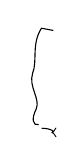
\begin{tikzpicture}[x=0.35cm,y=0.35cm]
\draw[thin] (0.45,3.5) -- (0.02,3.58) .. controls (-0.35,3.0) and (-0.12,2.4) .. (-0.30,1.95) .. controls (-0.46,1.45) and (-0.01,1.03) .. (-0.17,0.65) .. controls (-0.35,0.30) and (-0.30,0.03) .. (-0.08,0.08);
\draw[thin,->] (0.03,-0.05) .. controls (0.40,-0.05) and (0.52,-0.20) .. (0.38,-0.20);
\end{tikzpicture}}}}
\uline{Premier cas} : \handwritten{S}upposons d'abord $G$ algébrique. D'après (\deleted{\unsure{Exp.}} $\mathrm{VI}_A$ 3.2), le conoyau $K$ de l'injection $H\handwritten{\longrightarrow}G$ existe, \deleted{et} le morphisme canonique $p:G\handwritten{\longrightarrow}K$ est \deleted{fidèlement plat , et quasi-compact, puisque $G$ est de type fini sur $k$, et que $K$, qui est muni d'une structure de $k$-groupe (Exp. $\mathrm{VI}_A$ 5.2) est séparé sur $k$ (Exp. $\mathrm{VI}_A$ 0.2). Donc $p$ est} couvrant pour la topologie fpqc, \deleted{si bien (\deleted{\unsure{Exp.}} IV 4.4.3) que}\inserted{\handwritten{et}} $K$ représente le faisceau quotient $G/H$ pour la topologie fpqc;
